\begin{figure}[!htbp]
	\centering
	\resizebox{\textwidth}{!}{%
		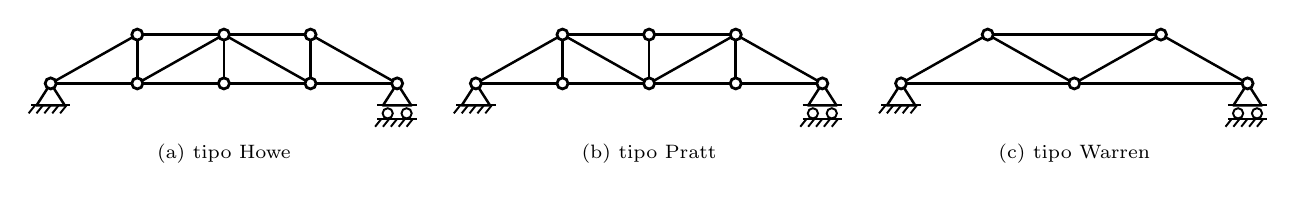
\begin{tikzpicture}[
			asta/.style={line width=0.90pt, line cap=round, line join=round, black},
			cord/.style={line width=0.90pt, line cap=round, line join=round, black},
			nodo/.style={circle, fill=white, draw=black, inner sep=0pt, minimum size=4pt, line width=1.0pt},
			terra/.style={line width=0.7pt, black},
			]
			
			
			\def\d{1.1}
			\def\h{0.62}
			
			%% ── (a) Pratt ──────────────────────────────────────────
			\begin{scope}[xshift=0cm]
				\draw[cord](0,0)--(4*\d,0);
				\draw[cord](\d,\h)--(3*\d,\h);
				\draw[asta](\d,0)--(\d,\h);
				\draw[asta](2*\d,0)--(2*\d,\h);
				\draw[asta](3*\d,0)--(3*\d,\h);
				\draw[asta](0,0)--(\d,\h);
				\draw[asta](\d,0)--(2*\d,\h);
				\draw[asta](3*\d,0)--(2*\d,\h);
				\draw[asta](4*\d,0)--(3*\d,\h);
				\draw[cord](0,0)--(-0.18,-0.28)--(0.18,-0.28)--cycle;
				\draw[terra](-0.25,-0.28)--(0.25,-0.28);
				\foreach \xx in {-0.20,-0.10,0,0.10,0.20}
				\draw[terra](\xx,-0.28)--++(-0.08,-0.10);
				\draw[cord](4*\d,0)--(4*\d-0.18,-0.28)--(4*\d+0.18,-0.28)--cycle;
				\draw[terra](4*\d-0.25,-0.28)--(4*\d+0.25,-0.28);
				\draw[terra](4*\d-0.12,-0.38)circle(0.065);
				\draw[terra](4*\d+0.12,-0.38)circle(0.065);
				\draw[terra](4*\d-0.25,-0.45)--(4*\d+0.25,-0.45);
				\foreach \xx in {-0.20,-0.10,0,0.10,0.20}
				\draw[terra](4*\d+\xx,-0.45)--++(-0.08,-0.10);
				\foreach \x in {0,1,2,3,4} \node[nodo]at(\x*\d,0){};
				\foreach \x in {1,2,3}     \node[nodo]at(\x*\d,\h){};
				\node[below,font=\scriptsize]at(2*\d,-0.65){(a) tipo Howe};
			\end{scope}
			
			%% ── (b) Howe ───────────────────────────────────────────
			\begin{scope}[xshift=5.4cm]
				\draw[cord](0,0)--(4*\d,0);
				\draw[cord](\d,\h)--(3*\d,\h);
				\draw[asta](\d,0)--(\d,\h);
				\draw[asta](2*\d,0)--(2*\d,\h);
				\draw[asta](3*\d,0)--(3*\d,\h);
				\draw[asta](0,0)--(\d,\h);
				\draw[asta](\d,\h)--(2*\d,0);
				\draw[asta](3*\d,\h)--(2*\d,0);
				\draw[asta](4*\d,0)--(3*\d,\h);
				\draw[cord](0,0)--(-0.18,-0.28)--(0.18,-0.28)--cycle;
				\draw[terra](-0.25,-0.28)--(0.25,-0.28);
				\foreach \xx in {-0.20,-0.10,0,0.10,0.20}
				\draw[terra](\xx,-0.28)--++(-0.08,-0.10);
				\draw[cord](4*\d,0)--(4*\d-0.18,-0.28)--(4*\d+0.18,-0.28)--cycle;
				\draw[terra](4*\d-0.25,-0.28)--(4*\d+0.25,-0.28);
				\draw[terra](4*\d-0.12,-0.38)circle(0.065);
				\draw[terra](4*\d+0.12,-0.38)circle(0.065);
				\draw[terra](4*\d-0.25,-0.45)--(4*\d+0.25,-0.45);
				\foreach \xx in {-0.20,-0.10,0,0.10,0.20}
				\draw[terra](4*\d+\xx,-0.45)--++(-0.08,-0.10);
				\foreach \x in {0,1,2,3,4} \node[nodo]at(\x*\d,0){};
				\foreach \x in {1,2,3}     \node[nodo]at(\x*\d,\h){};
				\node[below,font=\scriptsize]at(2*\d,-0.65){(b) tipo Pratt};
			\end{scope}
			
			%% ── (c) Warren ─────────────────────────────────────────
			\begin{scope}[xshift=10.8cm]
				\draw[cord](0,0)--(4*\d,0);
				\draw[cord](\d,\h)--(3*\d,\h);
				\draw[asta](0,0)--(\d,\h);
				\draw[asta](\d,\h)--(2*\d,0);
				\draw[asta](2*\d,0)--(3*\d,\h);
				\draw[asta](3*\d,\h)--(4*\d,0);
				\draw[cord](0,0)--(-0.18,-0.28)--(0.18,-0.28)--cycle;
				\draw[terra](-0.25,-0.28)--(0.25,-0.28);
				\foreach \xx in {-0.20,-0.10,0,0.10,0.20}
				\draw[terra](\xx,-0.28)--++(-0.08,-0.10);
				\draw[cord](4*\d,0)--(4*\d-0.18,-0.28)--(4*\d+0.18,-0.28)--cycle;
				\draw[terra](4*\d-0.25,-0.28)--(4*\d+0.25,-0.28);
				\draw[terra](4*\d-0.12,-0.38)circle(0.065);
				\draw[terra](4*\d+0.12,-0.38)circle(0.065);
				\draw[terra](4*\d-0.25,-0.45)--(4*\d+0.25,-0.45);
				\foreach \xx in {-0.20,-0.10,0,0.10,0.20}
				\draw[terra](4*\d+\xx,-0.45)--++(-0.08,-0.10);
				\foreach \x in {0,2,4} \node[nodo]at(\x*\d,0){};
				\node[nodo]at(\d,\h){};
				\node[nodo]at(3*\d,\h){};
				\node[below,font=\scriptsize]at(2*\d,-0.65){(c) tipo Warren};
			\end{scope}
			
	\end{tikzpicture}}
	\caption{Famiglie di maglie triangolari --- correnti paralleli.
		\emph{(a)}~Tipo Howe: montanti e diagonali interne
		convergenti verso l'alto al centro; le diagonali
		lavorano a compressione sotto carichi verticali
		applicati ai nodi del corrente superiore.
		\emph{(b)}~Tipo Pratt: orientamento invertito rispetto
		a Howe; le diagonali convergono verso il basso al
		centro, lavorano a trazione e i montanti a
		compressione.
		\emph{(c)}~Tipo Warren: sole diagonali alternate,
		senza montanti.}
	\label{fig:correnti_paralleli}
	\label{fig:correnti_paralleli}
\end{figure}
